% !TEX program = xelatex
% !TEX encoding = UTF-8 Unicode
% !TEX spellcheck = de_DE

%Dorkenwald, Soloninov
%Blatt 8

\documentclass{scrreprt}

% !TEX program = xelatex
% !TEX encoding = UTF-8 Unicode
% !TEX spellcheck = de_DE

%Dorkenwald, Soloninov

\usepackage{ blindtext,
		booktabs,
		color,
		nicefrac,
		polyglossia,
		setspace,
		xltxtra,
		yfonts,
		hyperref
		}

\usepackage{listings}				% @! 		
\usepackage{fontspec}  				% @!
\usepackage{media9}				% @! fur aufgabe 8.2.e
\usepackage{listings}
\usepackage{makeidx}

\setmainlanguage{german}
\setromanfont[Mapping=tex-text]{Linux Libertine O}
\setsansfont[Mapping=tex-text]{Linux Biolinum O}

\lstset{
         basicstyle=\footnotesize\ttfamily, 		% Standardschrift
         %numbers=left,               				% Ort der Zeilennummern
         numberstyle=\tiny,         				 % Stil der Zeilennummern
         %stepnumber=2,               				% Abstand zwischen den Zeilennummern
         numbersep=5pt,              				% Abstand der Nummern zum Text
         tabsize=2,                  % Groesse von Tabs
         extendedchars=true,         %
         breaklines=true,            % Zeilen werden Umgebrochen
         keywordstyle=\color{red},
            frame=b,         
 %        keywordstyle=[1]\textbf,    % Stil der Keywords
 %        keywordstyle=[2]\textbf,    %
 %        keywordstyle=[3]\textbf,    %
 %        keywordstyle=[4]\textbf,   \sqrt{\sqrt{}} %
         stringstyle=\color{white}\ttfamily, % Farbe der String
         showspaces=false,           % Leerzeichen anzeigen ?
         showtabs=false,             % Tabs anzeigen ?
         xleftmargin=17pt,
         framexleftmargin=17pt,
         framexrightmargin=5pt,
         framexbottommargin=4pt,
         %backgroundcolor=\color{lightgray},
         showstringspaces=false      % Leerzeichen in Strings anzeigen ?        
 }
 \lstloadlanguages{% Check Dokumentation for further languages ...
         %[Visual]Basic
         %Pascal
         %C
         %C++
         %XML
         %HTML
         Java
 }
    %\DeclareCaptionFont{blue}{\color{blue}} 

  %\captionsetup[lstlisting]{singlelinecheck=false, labelfont={blue}, textfont={blue}}
  \usepackage{caption}
\DeclareCaptionFont{white}{\color{white}}
\DeclareCaptionFormat{listing}{\colorbox[cmyk]{0.43, 0.35, 0.35,0.01}{\parbox{\textwidth}{\hspace{15pt}#1#2#3}}}
\captionsetup[lstlisting]{format=listing,labelfont=white,textfont=white, singlelinecheck=false, margin=0pt, font={bf,footnotesize}}
		% Header

\onehalfspacing
%path
\newcommand*{\Path}{./inhalte}

\makeindex

\begin{document}

	%add Schmutztitel
	\extratitle{Schmutztitel \\ Dorkenwald,Soloninov}

	%add Title
	\title{Titel des Dokumentes}
	\author{Dorkenwald,Soloninov}
	\date{10.12.2015}
	\maketitle

	%add Inhaltsverzeichnis
	\tableofcontents
	\newpage

	\subsection*{Abstract}
Dieses Dokument dient der Übung des Satzes von umfangreichen Projekten in \LaTeX\index{LaTeX@\LaTeX}. Es gehört zum achten Übungszettel des \LaTeX-Kurses im Wintersemester 	2015\,/\,16. Inhaltlich hat es so ziemlich nichts zu bieten, es könnte aber interessant sein, sich den zugehörigen Sourcecode mal anzusehen, da er eine Menge interessanter \LaTeX-Kommandos enthält.

	%add Path
	\setchapterpreamble[o]{\dictum[W. Busch]{Stets findet Überraschung statt. Da, wo man's nicht erwartet hat.}}

\chapter{Einleitung}

\blindtext$\sin(x)\cdot\cos(x) = -\nicefrac{1}{2} \cos(2x)$\footnote{Man baechte auch, dass $\sin(x\pm y) = \sin(x)\cos(y) \pm \cos(x)\sin(y)$}

\begin{table}[h]
  \centering
  \begin{tabular}{ccc}
    \toprule
    a & b & c\\
    d & e & f\\
    g & h & i\\
    \bottomrule
  \end{tabular}
  \caption{Die erste Tabelle}
  \label{tabelle1}
\end{table}
	\setchapterpreamble[o]{\dictum[Cato]{\textsc{Nullus est liber tam malus, ut non aliqua parte prosit.}}}

\index{Blinddokument|(}
\blinddocument
\index{Blinddokument|)}

\begin{figure}[h]
  \centering
  \fbox{I am a picture!}
  \caption{Ein Bild, das die Aussage des Textes unterstreicht.}
  \label{statement}
\end{figure}






\setchapterpreamble[o]{\dictum[U.\,R. Heber]{Ein schlauer Spruch bereichtert den Kapitelanfang.}}

\chapter{Ein weiteres Kapitel}

\fbox{I am a picture, introducing this chapter!}
\caption{Bildunterschrift}
\label{introduction}

\index{Blindtext}
\Blindtext\footnote{Man beachte auch, dass $\sin(x\pm y) = \sin(x)\cos(y) \pm \cos(x)\sin(y)$}

\begin{table}[h]
  \centering
  \begin{tabular}{ccc}
  \toprule
  eins & zwei & drei\\
  vier & fünf & sechs\\
  sieben & acht & neun\\
  \bottomrule
  \end{tabular}
  \caption{Eine Tabelle mit neun Einträgen}
  \label{tabelle3}
\end{table}
		
	\setchapterpreamble[o]{\dictum[F. Halm]{\hspace*{2em}\textfrak{Ruhe bleibt den Leichen;\\ Der Lebende tauch' frisch ins: Lebens:meer.}}}


\chapter{Und noch ein weiteres Kapitel}

\begin{figure}[p]
  \centering
  \fbox{I am a picture!}
  \caption{Beispiel zu diesem Kapitel}
  \label{example}
\end{figure}

\index{Blindtext}
\Blindtext 
Der \verb $\Bindtext$ - Befehl\index{Blindtext} ist eine nette Sache, wenn man\index{man} in \LaTeX\index{LaTeX@\LaTeX} sehen will, 
wie ein Dokument mit viel Inhalt aussieht, ohne, dass man Inhalt hat.

\begin{figure}[p]
  \centering
  \fbox{I am a picture!}
  \caption{Veranschaulichung der Aussage}
  \label{fig:illustration}				%add "fig:"
\end{figure}

\begin{figure}[p]
  \centering
  \fbox{I am a picture!}
  \caption{Detailansicht}
  \label{fig:detail}					%add "fig:"
\end{figure}

\begin{figure}[p]
  \centering
  \fbox{I am a picture!}
  \caption{Visualisierung des Ergebnisses}
  \label{fig:visualization}				%add "fig:"
\end{figure}
	
	%add Code
	Da sind die code fur aufgabe 8.2.d
	\lstinputlisting[label=RatedProvider,caption=A Provider for RatedMovies]{sourceCode/RatedMoviesContentProvider.java}
	\label{lst:RatedProvider}
	\lstinputlisting[label=MovieProvider,caption=A Provider for Movies]{sourceCode/MoviesContentProvider.java}
	\label{lst:MovieProvider}
	
	%add Somthing, Aufgabe 8.2.e
	\newpage
	Bei Korrektur wird es so : 

	\includemedia[activate=onclick,width=1 \textwidth]
	{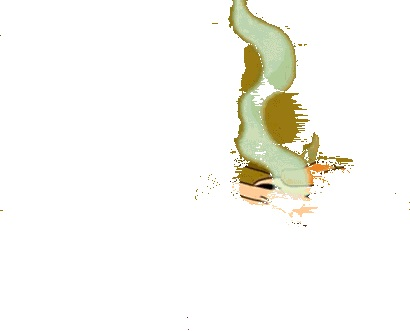
\includegraphics{./swf/my_tex_start.jpg}}{./swf/my_tex.swf}

	%appendix
	\begin{appendix}
		\chapter*{Anhang}
		\addcontentsline{toc}{chapter}{index}
		\printindex
		\addcontentsline{toc}{chapter}{Abbildungsverzeichnis}
		\listoffigures
		\addcontentsline{toc}{chapter}{Tabellenverzeichnis}
		\listoftables
		\addcontentsline{toc}{chapter}{List of Listings}
		\lstlistoflistings
	\end{appendix}

\end{document}	

